% TODO: THis reference
% REFERENCE https://forums.developer.nvidia.com/t/loop-through-register-array-without-using-local-memory/29458/3
\chapter{Local array optimization}

\label{sec:local_array_optimization}

% Why is it important that the arrays are in registers
% REFERENCE https://developer.nvidia.com/blog/fast-dynamic-indexing-private-arrays-cuda/
All \textit{multimat} and \textit{multirow} optimizations heavily rely on the ability of the CUDA compiler to place arrays such as the following into registers:

\begin{lstlisting}[
style=cuda
]
template<size_t LENGTH>
__device__ void foo(...) {
	...
	float bar[LENGTH];
	for (size_t i = 0; i < LENGTH; ++i) {
		bar[i] = some_function(...);
	}
	...
}
\end{lstlisting}

% TODO: Quote the blog
If an array is small and only accessed using static indexing, where all indices are known constants at compile time, the CUDA compiler places all elements of the array into registers \citep{site:private_arrays_cuda}. The array can also be accessed in small for loops with known compile time bounds, which are unrolled by the compiler and again result in static indexing. If for any access the index cannot be computed during compile time, the whole array is placed into Local memory, described in Section \ref{sec:memory_hierarchy}. Local memory is part of the device memory, and as such is the slowest memory accessible from device code. Local memory access also utilizes the same pipeline as warp shuffle instructions, competing for the throughput of this pipeline. 


\section{Advanced optimizations and local arrays}
\label{sec:local_array_optimization_code_changes}

While implementing the \textit{multimat\_both} and \textit{multirow\_both} optimizations, which are described in  Sections \ref{sec:multimat_both} and \ref{sec:multirow_both} respectively, we encountered a problem with the \textit{nvcc} compiler not optimizing the local arrays into registers. 

Using profiling and examining the SASS, we isolated the problem to the \textit{thread\_left\_bottom} and \textit{thread\_left\_top} arrays. We further isolated it to the following part of the code, which in its original form shared by the simplified, \textit{multimat\_right} and \textit{multirow\_right} implementations looks like this:

\begin{lstlisting}[
style=cuda
]
thread_left_bottom = warp.shfl(
	warp.thread_rank() != 0 ? thread_left_bottom : thread_left_top,
	warp.thread_rank() + 1
);
thread_left_top = warp.shfl_down(thread_left_top, 1);
\end{lstlisting}

To process multiple values from left input matrices, which is the basis of both \textit{multimat\_both} and \textit{multirow\_both} optimizations, the code needs to be changed into the following:

\begin{lstlisting}[
style=cuda
]
#pragma unroll
for (size_t l = 0; l < NUM_LEFTS; ++l) {
	thread_left_bottom[l] = warp.shfl(
		warp.thread_rank() != 0 ? thread_left_bottom[l] : thread_left_top[l],
		warp.thread_rank() + 1
	);
	thread_left_top[l] = warp.shfl_down(thread_left_top[l], 1);
}
\end{lstlisting}

The \textit{nvcc} compiler should be able to unroll this loop, and thanks to static indexing, the \textit{thread\_left\_bottom} and \textit{thread\_left\_top} local arrays should be optimized into registers. Unfortunately, as we can see in Listing \ref{lst:sass_local_mem}, the compiler behaves as if dynamic indexing was used and pushes the arrays into local memory. 
Due to the closed source nature of the \textit{nvcc} compiler, we can only speculate on the reasons why the loop unrolling does not result in static indexing. One possibility, based on the generated SASS instructions seen in Listing \ref{lst:sass_local_mem}, is that the ternary operator is optimized into dynamic array indexing, which then prevents the local array optimization. As there is no visible branching in the unrolled loop, the base address of either the \textit{thread\_left\_bottom} or the \textit{thread\_left\_top} is loaded into register R63, which is then reused in all loads, resulting in dynamic indexing. 

% TODO: Add coloring
\begin{lstlisting}[
style=sass,
caption={SASS instructions without local array optimization},
label=lst:sass_local_mem
]
LDL R0, [R63+0x4]
SHFL.IDX PT, R8, R0, R57, 0x1f
SHFL.DOWN PT, R0, R32, 0x1, 0x1f
STL [R62], R8
STL [R61], R0
\end{lstlisting}

We experimented with several solutions, with the following version compiling into static indexing:

\begin{lstlisting}[
style=cuda
]
#pragma unroll
for (size_t l = 0; l < NUM_LEFTS; ++l) {
	T bottom_shift_val;
	if (warp.thread_rank() != 0) {
		bottom_shift_val = thread_left_bottom[l];
	} else {
		bottom_shift_val = thread_left_top[l];
	}

	thread_left_bottom[l] = warp.shfl(bottom_shift_val, warp.thread_rank() + 1);
	thread_left_top[l] = warp.shfl_down(thread_left_top[l], 1);
}
\end{lstlisting}

% TODO: Add coloring
\begin{lstlisting}[
style=sass,
caption={SASS instructions with local array optimization},
label=lst:sass_no_local_memory
]
SEL R42, R52, R20, !P4
SHFL.IDX PT, R53, R48, R53, 0x1f
SHFL.DOWN PT, R52, R52, 0x1, 0x1f
\end{lstlisting}

The only change is the expansion of the ternary operator into an equivalent if statement. As shown in Listing \ref{lst:sass_no_local_memory}, the body of the updated loop results in a single \textit{SEL} instruction which selects the top or the bottom part of the buffer. This version of the loop is used by the \textit{multimat\_both} and \textit{multirow\_both} optimizations described in the following sections.

The difference is also visible in Figure \ref{fig:instruction_mix_local_mem}, which shows the additional local memory store (STL) and load (LDL) instructions in both the \textit{multimat\_both} and \textit{multirow\_both} without local array optimization. Apart from these additional instructions, the number of remaining instructions is generally the same, with some additional integer multiply-add instructions (IMAD) in Figure \ref{fig:local_mem_multimat_both_instruction_mix} due to local memory address computations.

\begin{figure}[ht]
	\centering	
	\begin{subfigure}{\textwidth}
		\centering
		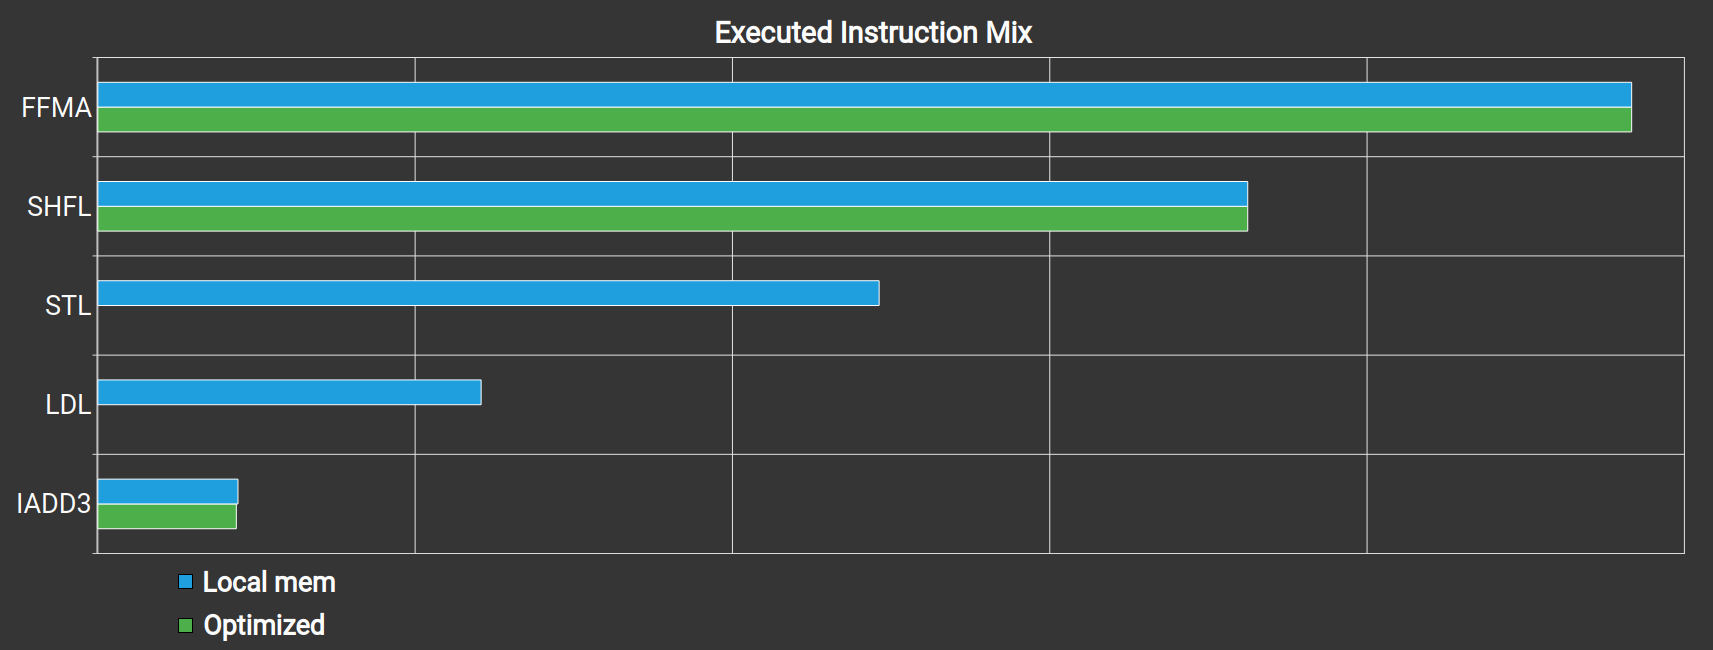
\includegraphics[width=0.7\textwidth]{executed_instructions_shuffle_multimat_both.png}
		\caption{The \textit{multimat\_both} optimization.}
		\label{fig:local_mem_multimat_both_instruction_mix}
	\end{subfigure}
	\hfill
	\begin{subfigure}{\textwidth}
		\centering
		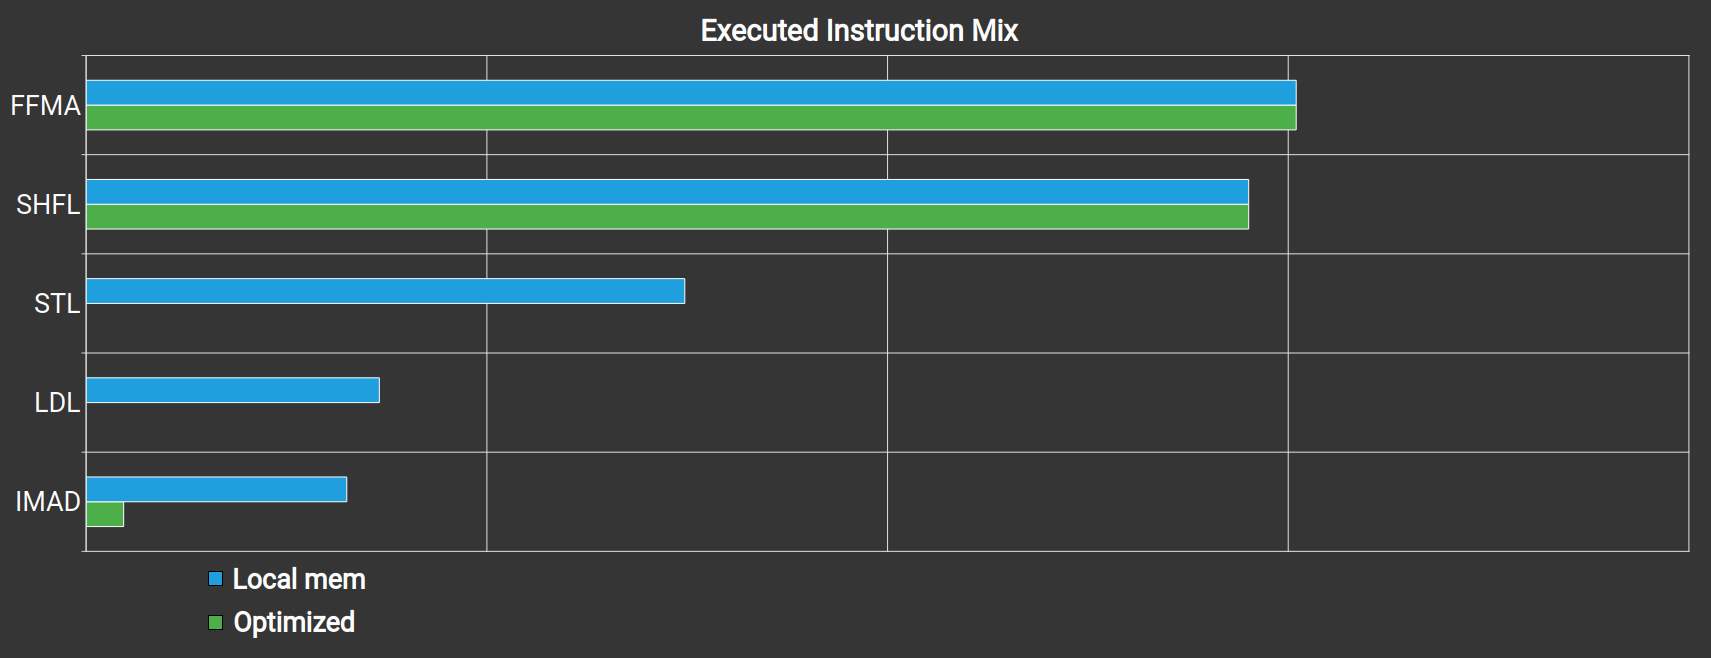
\includegraphics[width=0.7\textwidth]{executed_instructions_shuffle_multirow_both.png}
		\caption{The \textit{multirow\_both} optimization.}
		\label{fig:local_mem_multirow_both_instruction_mix}
	\end{subfigure}
	
	\caption{Comparison of the instruction mix between a version with arrays in local memory and a version with arrays in registers.}
	\label{fig:instruction_mix_local_mem}
\end{figure}

Based on this observation, the measured speedup in Figure \ref{fig:speedup_local_mem} is caused solely by the application of the local array optimization. The speedup for smaller inputs is limited due to low occupancy, but is still present. As an example, Figure \ref{fig:multimat_both_speedup} shows that for input matrices of size 64 by 64, the solution without local memory access is already 2 times faster. Figure \ref{fig:multirow_both_speedup} shows that there is slightly smaller improvement in the \textit{multirow\_both} optimization compared to the \textit{multimat\_both}. This is most likely caused by higher general overhead due to the greater overall complexity of the optimization.


\begin{figure}[ht]
	\centering	
	\begin{subfigure}{0.45\textwidth}
		\centering
		\def\svgwidth{\textwidth}
		% Must be relative to current directory
		% as input ignores graphicspath, which is
		% only for includegraphics{}
		\input{./img/multimat_speedup.pdf_tex}
		\caption{The \textit{multimat\_both} optimization.}
		\label{fig:multimat_both_speedup}
	\end{subfigure}
	\hfill
	\begin{subfigure}{0.45\textwidth}
		\centering
		\def\svgwidth{\textwidth}
		% Must be relative to current directory
		% as input ignores graphicspath, which is
		% only for includegraphics{}
		\input{./img/multirow_speedup.pdf_tex}
		\caption{The \textit{multirow\_both} optimization.}
		\label{fig:multirow_both_speedup}
	\end{subfigure}
	
	\caption{Improvement of the two optimizations without local memory access.}
	\label{fig:speedup_local_mem}
\end{figure}



\chapter{User guide}
This section first describes the process of building and running the CUDA C++ program implementing the definition-based, FFT-based and simple CPU-based cross-correlation algorithms, together with result validation. Next we illustrate the usage of benchmarking tool implemented to simplify validation and benchmarking of the CUDA C++ program.

\section{Building the CUDA C++ program}
The CUDA C++ program has following dependencies:
\begin{itemize}
	\item CMake 3.18 or newer,
	\item CUDA 11.4 or newer,
	\item (Optional) Boost 1.71 or newer,
	\item (Optional) nlohmann/json 3.7.3 or newer
\end{itemize}

Optional dependencies can either be provided externally or downloaded automatically using a CMake superbuild. To build the program with externally provided optional dependencies, follow these steps:
\begin{enumerate}
	\item go to the project repository root directory
	\item \texttt{mkdir build \&\& cd build}
	\item \texttt{cmake ..}
	\item \texttt{cmake --build .}
\end{enumerate}

The build was tested on Ubuntu 20.04 and Rocky Linux 8.5.
Most implementations allow customizing limits, such as maximum number of overlaps (shifts) grouped into a job, number of right input matrices to process overlaps from in a single job, or number rows from the left input matrix processed in a single iteration. Following is the full list of provided options with their default values for Release/Debug build. The structure of the option name is \textit{\textlangle algorithm\_name \textrangle \textlangle limit\_name\textrangle}.

% TODO: Remove this
\begin{center}
	\begin{tabular}{|l|c|c|} 
		\hline
		Option name&Release&Debug\\ [0.5ex] 
		\hline\hline
		SHUFFLE\_MULTIMAT\_RIGHT\_RIGHT\_MATRICES\_PER\_THREAD\_LIMIT&8&4\\
		\hline
		SHUFFLE\_MULTIROW\_RIGHT\_RIGHT\_ROWS\_LIMIT&8&4\\
		\hline
		SHUFFLE\_MULTIROW\_BOTH\_SHIFTS\_PER\_THREAD\_LIMIT&8&4\\
		\hline
		SHUFFLE\_MULTIROW\_BOTH\_LEFT\_ROWS\_LIMIT&4&2\\
		\hline
		SHUFFLE\_MULTIROW\_BOTH\_LOCAL\_MEM\_SHIFTS\_PER\_THREAD\_LIMIT&4&2\\
		\hline
		SHUFFLE\_MULTIROW\_BOTH\_LOCAL\_MEM\_LEFT\_ROWS\_LIMIT&4&2\\
		\hline
		SHUFFLE\_MULTIROW\_RIGHT\_MULTIMAT\_RIGHT\_RIGHT\_ROWS\_LIMIT&4&2\\
		\hline
		SHUFFLE\_MULTIROW\_RIGHT\_MULTIMAT\_RIGHT\_RIGHT\_MATS\_LIMIT&4&2\\
		\hline
		SHUFFLE\_N\_TO\_M\_MULTIMAT\_BOTH\_LEFT\_MATRICES\_PER\_THREAD\_LIMIT&4&2\\
		\hline
		SHUFFLE\_N\_TO\_M\_MULTIMAT\_BOTH\_RIGHT\_MATRICES\_PER\_THREAD\_LIMIT&4&2\\
		\hline
		SHUFFLE\_N\_TO\_M\_MULTIMAT\_BOTH\_LOCAL\_MEM\_LEFT\_MATRICES\_PER\_THREAD\_LIMIT&4&2\\
		\hline
		SHUFFLE\_N\_TO\_M\_MULTIMAT\_BOTH\_LOCAL\_MEM\_RIGHT\_MATRICES\_PER\_THREAD\_LIMIT&4&2\\
		\hline
		SHUFFLE\_N\_TO\_M\_MULTIROW\_BOTH\_MULTIMAT\_BOTH\_SHIFTS\_PER\_THREAD\_PER\_RIGHT\_MATRIX\_LIMIT&4&2\\
		\hline
		SHUFFLE\_N\_TO\_M\_MULTIROW\_BOTH\_MULTIMAT\_BOTH\_RIGHT\_MATRICES\_PER\_THREAD\_LIMIT&4&2\\
		\hline
		SHUFFLE\_N\_TO\_M\_MULTIROW\_BOTH\_MULTIMAT\_BOTH\_LEFT\_MATRICES\_PER\_THREAD\_LIMIT&4&2\\
		\hline
		SHUFFLE\_N\_TO\_M\_MULTIROW\_BOTH\_MULTIMAT\_BOTH\_LEFT\_ROWS\_PER\_ITERATION\_LIMIT&4&2\\
		\hline
		SHUFFLE\_ONE\_TO\_MANY\_MULTIROW\_BOTH\_MULTIMAT\_RIGHT\_SHIFTS\_PER\_RIGHT\_MATRIX\_LIMIT&4&2\\
		\hline
		SHUFFLE\_ONE\_TO\_MANY\_MULTIROW\_BOTH\_MULTIMAT\_RIGHT\_RIGHT\_MATRICES\_PER\_THREAD\_LIMIT&4&2\\
		\hline
		SHUFFLE\_ONE\_TO\_MANY\_MULTIROW\_BOTH\_MULTIMAT\_RIGHT\_LEFT\_ROWS\_PER\_ITERATION\_LIMIT&4&2\\
		\hline
		WARP\_PER\_SHIFT\_SHARED\_MEM\_RIGHT\_MATRICES\_PER\_BLOCK\_LIMIT&8&2\\
		\hline
	\end{tabular}
\end{center}

Use CMake GUI or a \texttt{-D} option in step 3 to change the Release value. The values of these options greatly influence the build time of the program. With the default settings listed above, the build time is over 8 hours, mainly limited by the \texttt{SHUFFLE\_N\_TO\_M\_MULTIROW\_BOTH\_MULTIMAT\_BOTH} and \texttt{SHUFFLE\_ONE\_TO\_MANY\_MULTIROW\_BOTH\_MULTIMAT\_RIGHT} algorithms. Feel free to change the values to speed up the build time in exchange for limiting the range of runtime arguments and consequently limiting the maximum speed of the algorithm.
To download the optional dependencies automatically during the build, add \texttt{-D USE\_SUPERBUILD=ON} option to the command in step 3. 
The output of the build should be \textit{cross} executable in the build directory.

% TODO: Maybe mention the script to build on gpulab
\section{Running the CUDA C++ program}
The \textit{cross} executable implements the following commands:

\begin{itemize}
	\item[help] Prints help message describing the CLI interface.
	\item[run] Runs a computation using the specified algorithm, optionally writing the output to a file, measuring execution times or validating the output. 
	
	Positional arguments:
	\begin{enumerate}
		\item \texttt{alg} The algorithm to use for the computation,
		\item \texttt{ref\_path} The path to the left input matrix/matrices,
		\item \texttt{target\_path} The path to the right input matrix/matrices.
	\end{enumerate}

	Options and switches:
	\begin{itemize}
		\item \texttt{-d,--data\_type \textlangle"single" \textbar  "double"\textrangle} Data type to use for computation, choice between single and double floating point numbers, defaults to single;
		\item \texttt{-o,--out \textlangle path\textrangle} Path to the output file for the result of the computation which is only stored if this option is provided;
		\item\texttt{-t,--times \textlangle path\textrangle} Path to the file in which to store the measured execution times;
		\item \texttt{-v,--validate \textbraceleft path\textbraceright} Option with an optional value which either enables validation against valid results computed using simple CPU implementation, or additionally provides a path to valid results to use for comparison. Validation results are written to the standard output;
		\item \texttt{-n,--normalize} If results of FFT-based algorithm should be normalized before being written to the output file. Ignored if not writing output or if algorithm is not FFT-based;
		\item \texttt{-a,--append} Append times to the file instead of overwriting it;
		\item \texttt{-p,--no\_progress} Do not print computation progress to standard output;
		\item \texttt{-b,--benchmark\_type \textlangle"Compute"\textbar"CommonSteps"\textbar"Algorithm"\textbar"None"\textrangle} Which part of the implementation should be measured, defaults to \texttt{Compute};
		\item \texttt{-l,--outer\_loops} Number of times the algorithm should be run after loading the data into memory. Each run is measured separately;
		\item \texttt{-m,--min\_time} Minimum measurement time for measurements with adaptive iteration count, defaults to 1 second;
		\item \texttt{--args\_path} Path to the JSON file containing argument values for the algorithm.
	\end{itemize}
	\item[list] Lists the available algorithms. Each of the listed names can be used as \textit{alg} positional argument of the \textit{run} command. 
	\item[validate] Compares two result files, executing the same validation as optionally done by the \textit{run} command on the output of the computation.
	
	Positional arguments:
	\begin{enumerate}
		\item \texttt{template\_data\_path} The path to the known correct output to compare against,
		\item \texttt{validate\_data\_path} The path to the data to be validated.
	\end{enumerate}

	Options and switches:
	\begin{itemize}
		\item \texttt{-n,--normalize} Normalize validated data. This option is useful when results of FFT-based algorithm were stored without normalization;
		\item \texttt{-c,--csv} Print output in CSV format instead of in human readable format;
		\item \texttt{-p,--print\_header} Print header before the output data. Useful when not appending to existing file.
	\end{itemize}
	\item[input] Validate that the given input matrices can be computed by given algorithm.
	
	Positional arguments:
	\begin{enumerate}
		\item \texttt{alg\_type} The algorithm to validate for,
		\item \texttt{rows} The number of rows of each input matrix,
		\item \texttt{cols} The number of columns of each input matrix,
		\item \texttt{left\_matrices} The number of left input matrices,
		\item \texttt{right\_matrices} The number of right input matrices.
	\end{enumerate}
\end{itemize}

\section{Using the benchmarking tool}
The benchmarking tool is a Python CLI application designed to simplify running large number of benchmarks or validations using the \texttt{cross} executable or any of the existing cross-correlation implementations, in the version of the code attached to this thesis using SciPy or Matlab. The tool is designed to install all dependencies using \textit{poetry} and to run the \texttt{benchmarking.py} script, providing the following commands:

\begin{itemize}
% TODO: List arguments
	\item
\end{itemize}

For an example of benchmark definition, see \texttt{benchmarking/example\_benchmark.yml} file or any of the benchmark definitions used for gathering data showcased in this thesis in \texttt{benchmarking/text}. 
\chapter{Attachments}